\documentclass[11pt]{article}

\usepackage[margin=1in]{geometry}
\usepackage[T1]{fontenc}
\usepackage[utf8]{inputenc}
\usepackage{lmodern}
\usepackage{amsmath,amssymb}
\usepackage{booktabs}
\usepackage{graphicx}
\usepackage{xcolor}
\usepackage{algorithm}
\usepackage{algpseudocode}
\usepackage[round,authoryear]{natbib}
\usepackage{xurl}
\usepackage[colorlinks=true,linkcolor=blue!50!black,citecolor=blue!50!black,urlcolor=blue!50!black]{hyperref}

\newcommand{\sherpa}{\textsc{sherpa}}

\title{\sherpa: Joint Estimation of Used Heavy-Equipment Sale Prices and Rental Rates from Sparse Marketplace Listings}

\author{EquipmentsFinder\\
\small\url{https://www.equipmentsfinder.com}}

\date{October 2026 \quad (preprint, version 1)}

\begin{document}

\maketitle

\begin{abstract}
Online marketplaces for construction and industrial machinery publish asking prices for sale and
asking rates for hire, but their listings are few per category, often incomplete, and noisy. We
present \sherpa{} (Shrinkage-based Heavy Equipment Residual Price Analysis), an explainable model
that fits sale prices and rental rates \emph{jointly}: both are treated as observations of one
underlying machine value, built from a flexible Box--Cox depreciation curve, size, usage relative to
age, condition, attachments, seller type, a brand-to-origin hierarchy and further listing
attributes. The rental side adds a per-category rent-to-value level, motivated by the user cost of
capital, a duration discount under which the rate per day falls as a power of hire length, and an
operator premium. Every effect is estimated robustly (medians and Theil--Sen slopes) by backfitting
with empirical-Bayes partial pooling and domain constraints, stabilised by averaging the iterates,
and every estimate carries a cross-conformal prediction interval calibrated separately for listings
with missing inputs. In a simulation study on synthetic markets with known parameters, \sherpa{}
recovers the parameters it was given and is the most accurate model at every market size: with 20
listings per category and side it reduces the median absolute percentage error of sale-price
estimates from 45\% for an ordinary least-squares hedonic regression to 31\%, and of rental rates
from 50\% to 28\%. It is insensitive to impossible prices that more than double the regression's
error, fitting rental listings jointly cuts sale-price error by up to 11 percentage points when
sales are scarce, and its conformal intervals stay conservative in small markets where normal
intervals under-cover. The model is released as open-source software in TypeScript and Python.
\end{abstract}

\section{Introduction}

What is a ten-year-old 20-tonne excavator worth, and what should it rent for by the day, the week
or the month? Contractors, rental companies, lenders and insurers ask these questions daily. The
academic literature on the residual value of heavy equipment answers the first from auction
records with clean, structured fields \citep{lucko2006,fan2008,milosevic2021}; the second is
usually answered by rules of thumb from trade rate guides. Neither setting matches the data most
regional equipment markets actually produce: listings on an online marketplace, where a category
may have a few dozen priced machines, the manufacture year sits in the title if anywhere, engine
hours are rarely given, and a placeholder price of 1 or a monthly rate typed into the sale field is
common.

This paper presents \sherpa, a model built for that data. Its premise is that a sale listing and a
rental listing of the same kind of machine are two observations of one underlying value: the
rental rate is the price of using the machine for a while, and capital theory links it to the value
of the machine through the user cost of capital \citep{jorgenson1963,hall1967}. Fitting both
together lets a market with many rental listings and few sales still learn how age, size, condition
or brand move value, and the reverse.

\paragraph{Contributions.}
\begin{enumerate}
  \item A hedonic model with \emph{one machine-value core identified by two equations}, one for sale
  prices and one for rental rates, with a per-category rent-to-value level, a power-law duration
  discount and an operator premium on the rental side (Section~\ref{sec:model}).
  \item An estimation procedure for sparse, messy listings: robust backfitting with partial pooling
  over a category-family and brand-origin hierarchy, sign and monotonicity constraints, an
  identification strategy that prevents the sale and rent levels from drifting together, and
  averaging of the iterates for a stable answer (Section~\ref{sec:estimation}).
  \item Cross-conformal prediction intervals calibrated separately by side and by the number of
  missing inputs (Section~\ref{sec:intervals}).
  \item A simulation study with known parameters: recovery, accuracy against ordinary least
  squares and a simpler baseline, robustness to impossible prices and missing fields, the value of
  rental listings for sale estimates, interval calibration and ablations (Section~\ref{sec:results}).
  \item Open-source TypeScript and Python implementations without dependencies, kept equal by a
  cross-language test (Section~\ref{sec:software}).
\end{enumerate}

All experiments use synthetic markets, so that every estimate can be compared with the truth. A
case study on real marketplace listings is left to a later version of this paper.

\section{Related work}
\label{sec:related}

\paragraph{Residual value of machinery.}
Statistical models of the residual value of heavy construction equipment go back to
\citet{lucko2006} and \citet{lucko2007}, who regressed auction prices on age, hours and economic
conditions, revisited after the 2008 recession by \citet{lucko2011}. \citet{fan2008} used
regression trees; more recent work applies ensembles and neural networks to large sets of auction
or dealer records \citep{shehadeh2021,alshboul2021,milosevic2021,toma2024}, with
\citet{huymajer2025} cautioning against their pitfalls, and \citet{chiteri2018} relating residual
value to equipment cash flows. In agriculture, remaining-value functions for tractors and
implements have a long history \citep{cross1995,cross1996,dumler2003,wu2004} and inform the ASABE
D497 standard \citep{asabe_d497}; \citet{herranz2023,herranz2024} revisit them for European
tractors. These models price sales only, and none reports calibrated intervals.

\paragraph{Depreciation and functional form.}
\citet{hulten1981} estimated economic depreciation from vintage asset prices with Box--Cox forms
\citep{box1964}, letting the data choose between geometric, linear and concave patterns;
\citet{wu2004} compared functional forms for farm machinery and \citet{halvorsen1981} for hedonic
equations generally. \sherpa{} adopts a Box--Cox curve in age with a shape parameter per category.

\paragraph{Hedonic prices and rents.}
Hedonic regression \citep{rosen1974} and regression price indices \citep{bailey1963} are the
standard tools for pricing differentiated goods over time. Joint attention to prices and rents
comes mostly from housing: \citet{bracke2015} matches London homes that were both sold and rented,
\citet{hill2016} compare hedonic price--rent ratios with the user cost, and \citet{crone2004} and
\citet{garner2009} relate owner and rental costs. In vehicles, \citet{cho2010} study how rental
prices of cars depend on age and mileage. \citet{guasch1987} document a length-of-residency discount
in rents, the housing analogue of the hire-duration discount modelled here. We found no published
model that fits sale prices and rental rates of used equipment jointly with one shared value
function, nor a data-driven estimate of the duration discount for equipment; trade guides state
such multipliers as rules of thumb.

\paragraph{Seller type.}
Used-car markets show systematic dealer premiums \citep{genesove1993,emons2009,biglaiser2020}, which
vary with the type of intermediary \citep{li2025}. \sherpa{} includes seller type as a level effect.

\paragraph{Shrinkage.}
Pulling small-group estimates toward a parent is the empirical-Bayes idea of
\citet{james1961} and \citet{efron1973,efron1975}, used in small-area estimation
\citep{fay1979}, multilevel regression \citep{gelman2007}, house-price models
\citep{brunauer2013,gelfand2004,goodman2003} and target encoding of high-cardinality categories
\citep{miccibarreca2001}.

\paragraph{Robust estimation.}
\sherpa{} relies on medians, the Theil--Sen slope \citep{theil1950,sen1968}, the median absolute
deviation as a scale \citep{hampel1974,rousseeuw1993}, and the robustness ideas of
\citet{huber1964}, fitted by backfitting \citep{hastie1986,hastie1990} with averaged iterates
\citep{polyak1992}.

\paragraph{Prediction intervals.}
Conformal prediction gives distribution-free intervals \citep{vovk2005,lei2018}, with
cross-validation variants analysed by \citet{barber2021} and quantile-based variants by
\citet{romano2019}. Normalised nonconformity scores have been applied to automated valuation of
real estate \citep{bellotti2017,lim2021,bastos2025,hjort2025}; we are not aware of applications to
equipment prices.

\section{Model}
\label{sec:model}

\subsection{Data}
A listing $i$ is either a sale, with an asking price $P_i$, or a rental, with an asking rate for a
hire of $T_i$ days (a daily, weekly or monthly rate). It describes a machine of category $c$ in
family $f(c)$ by any subset of: brand $b$ and its origin group $o(b)$, manufacture year (hence age
$a$), size $s$ in the category's unit (tons, kVA), engine hours $h$, new or used, a condition grade
$q\in\{1,2,3,4\}$, a set of attachments $A$, an emissions standard $e$, the remaining life of wear
parts $w\in[0,1]$, a spec or import status $g$, a seller type $k$, an inspection flag $v$, a region
$r$, the listing month $t$, months on the market $m$ and a completeness score $\ell$. Every field
except the category, the side and the price may be missing. One model is fitted per market.

\subsection{Machine value}
The log value of machine $x$ is a sum of named effects around a reference machine of category $c$
(median age and size, used, good condition, no attachments):
\begin{align}
V(x) ={}& \alpha_c + \beta_c\,\bigl(g_{\lambda_c}(a) - g_{\lambda_c}(a^\star_c)\bigr)
        + \gamma_c \log\frac{s}{s^\star_c} + \delta_c\,u(h,a) + \theta_c\,\mathbf{1}[\text{new}]
        + \eta_q + \sum_{j\in A}\psi_j \nonumber\\
      & + \varepsilon_e + \zeta_c\,(w-\tfrac12) + \varphi_g + \kappa_k + \nu\,v
        + b_{o(b)} + b_b + b_{b,c} + \rho_r + \tau_t . \label{eq:value}
\end{align}
The depreciation curve is a Box--Cox transform of age,
\begin{equation}
g_\lambda(a) = \frac{(1+a)^\lambda - 1}{\lambda},\qquad g_0(a) = \log(1+a),\qquad \lambda\in[-1,1],
\end{equation}
which is linear in age (geometric depreciation) at $\lambda=1$ and front-loaded for smaller
$\lambda$. Usage enters relative to what is normal for the age,
\begin{equation}
u(h,a) = \log\frac{h + h_0}{\bar h_c \max(a,\tfrac12) + h_0},
\end{equation}
with $\bar h_c$ the category's typical annual hours and $h_0=250$, so that hours do not duplicate
the age effect. Categorical sets without a natural reference level (emissions, spec, seller, origin,
region) include an explicit \emph{unknown} level and are centred on the average listing; grade is
referenced at ``good'' ($\eta_3=0$).

Domain knowledge enters as constraints: machines lose value with age ($\beta_c<0$), larger machines
cost more ($\gamma_c\ge0$), more usage and worse condition never raise the price
($\delta_c\le0$, $\eta_1\le\eta_2\le\eta_3\le\eta_4$), and new machines and attachments never
lower it ($\theta_c\ge0$, $\psi_j\ge0$).

\subsection{Sale and rent equations}
Sale prices and rental rates share $V$:
\begin{align}
\log P_i &= V(x_i) + \lambda_m \log(1+m_i) + \lambda_\ell(\ell_i - \tfrac12) + \epsilon^{\text{sale}}_i,
  \label{eq:sale}\\
\log R_i(T_i) &= V(x_i) + \pi_c + \kappa_c \log\frac{T_i}{30} + \omega_c\,\mathbf{1}[\text{operator}]
  + \lambda_m \log(1+m_i) + \epsilon^{\text{rent}}_i , \label{eq:rent}
\end{align}
where $R_i(T)$ is the asking rate per day for a hire of $T$ days. The listing terms describe the
listing, not the machine, and are set to their reference values when a machine is valued.

$\pi_c$ is the log rate per day per unit of value at a one-month hire. Capital theory prices the use
of an asset by its user cost, $c = q\,(r + \delta) - \dot q$ for an asset of price $q$, interest
rate $r$ and depreciation rate $\delta$ \citep{jorgenson1963,hall1967}; categories that wear fast or
stand idle between hires therefore rent dearer relative to their value. $\kappa_c\le0$ is the
duration discount: the rate per day for a $T$-day hire is $R(T) = R(30)\,(T/30)^{\kappa_c}$, so one
parameter per category turns a daily rate into weekly and monthly ones. $\omega_c\ge0$ is the
premium for a wet hire with an operator.

\subsection{Hierarchy}
Every group estimate is shrunk toward its parent by partial pooling,
\begin{equation}
\hat\theta_{\text{group}} = \frac{n}{n+k}\,\tilde\theta_{\text{group}} + \frac{k}{n+k}\,\hat\theta_{\text{parent}},
\end{equation}
where $\tilde\theta$ is the group's own robust estimate from $n$ listings and $k$ the number of
listings at which group and parent weigh equally. Table~\ref{tab:hierarchy} lists the structure.

\begin{table}[t]
\centering\small
\caption{Hierarchy, default shrinkage strengths and constraints.}
\label{tab:hierarchy}
\begin{tabular}{lllcl}
\toprule
Parameter & Group & Parent & $k$ & Constraint \\
\midrule
$\alpha$ & category & family & 6 & -- \\
$D=\beta g_\lambda(H)$, $\lambda$ & category & pooled & 12, 24 & $D<0$, $\lambda\in[-1,1]$ \\
$\gamma$, $\delta$, $\zeta$ & category & pooled & 12 & $\gamma\ge0$, $\delta\le0$, $\zeta\ge0$ \\
$\theta$ & category & pooled & 10 & $\theta\ge0$ \\
$\eta_q$ & grade & 0 & 8 & monotone \\
$\psi_j$ & attachment & 0 & 6 & $\psi\ge0$ \\
$\varepsilon,\varphi,\kappa_k,\rho$ & level & 0 & 8 & centred \\
$b_o$, $b_b$, $b_{b,c}$ & origin, brand, brand$\times$category & 0 & 6, 4, 6 & centred ($b_o$) \\
$\pi$, $\kappa$, $\omega$ & category & pooled & 8 & $\kappa\le0$, $\omega\ge0$ \\
$\sigma$ & category$\times$side & pooled & 8 & $\sigma\ge0.1$ \\
\bottomrule
\end{tabular}
\end{table}

\section{Estimation}
\label{sec:estimation}

\sherpa{} is fitted by robust backfitting (Algorithm~\ref{alg:fit}): each block of parameters is
re-estimated on the partial residuals of all the others, using only medians and Theil--Sen slopes,
then shrunk and clamped.

\begin{algorithm}[t]
\caption{Fitting \sherpa}
\label{alg:fit}
\begin{algorithmic}[1]
\State Drop non-positive prices and log prices more than $3.5$ robust standard deviations from the
median of their category and side (rates put on a 30-day footing first).
\State Initialise $\alpha_c$ at the median sale log price, $\pi_c$ at the rent--sale median gap.
\For{round $=1,\dots,40$}
  \For{each block $B$ in turn}
    \State $\tilde y_i \gets y_i - \sum_{B'\neq B}\text{term}_{B'}(x_i)$ \Comment{partial residuals}
    \State estimate $B$ by medians or Theil--Sen slopes of $\tilde y$; shrink; clamp
  \EndFor
  \State centre the reference-free level sets and the time index; move each shift into $\alpha_c$
  \State \textbf{if} no prediction moved by more than $10^{-4}$ \textbf{then} stop
  \State \textbf{if} round $\ge 15$ \textbf{then} add all parameters to a running average
\EndFor
\State Set the parameters to their average over the rounds after the burn-in.
\State $\sigma_{c,\text{side}} \gets$ $1.4826\times$ MAD of residuals, shrunk to the pooled scale.
\State Calibrate intervals by cross-conformal scores (Section~\ref{sec:intervals}).
\end{algorithmic}
\end{algorithm}

\paragraph{Identification of the two levels.}
$\alpha_c$ and $\pi_c$ are separately identified only where a category has both sale and rental
listings. We estimate $\alpha_c$ from sale listings alone wherever a category has at least three,
and $\pi_c$ from rental listings given $\alpha_c$; elsewhere $\pi_c$ takes its pooled value.
Estimating $\alpha_c$ from both sides let $\alpha_c$ and $\pi_c$ slide along a ridge: the
shrinkage of $\pi_c$ toward the pooled value pulled it down a little each round, $\alpha_c$ rose to
compensate through the rental listings, and sale listings ended up over-predicted.

\paragraph{The depreciation curve.}
$\beta_c$ changes its units with $\lambda_c$, so the shrunk quantity is the depreciation at a fixed
horizon, $D_c=\beta_c\,g_{\lambda_c}(H)$ with $H=10$ years. $\lambda_c$ is chosen by profiling the
$L_1$ fit of a Theil--Sen line over a grid in $[-1,1]$, refined by a parabola through the best
grid point and its neighbours, during the first five rounds only, and then held fixed.

\paragraph{Averaging.}
Backfitting with median updates is not guaranteed to converge. In our experiments it reached the
neighbourhood of a fixed point and then wandered around it by about $\pm0.8\%$ in prediction
indefinitely; its answer depended on the round at which it stopped. Averaging the iterates after a
burn-in, as in stochastic approximation \citep{polyak1992}, fixes the answer and reduces the
round-to-round movement about tenfold.

\subsection{Prediction intervals}
\label{sec:intervals}
For an interval at level $1-\alpha$, the listings are split into $K$ folds; each fold is predicted
by a model fitted on the others, and its normalised scores
$S_i = |\log y_i - \log\hat y_i| / \hat\sigma_{c,\text{side}}$ are pooled by side and by the number of
missing price-moving inputs (year, size, hours, grade: 0, 1, or 2 or more), a Mondrian split. The
interval is $\hat y\exp(\pm\hat q\,\hat\sigma)$ with $\hat q$ the $\lceil(n+1)(1-\alpha)\rceil$-th
smallest score of the group \citep{vovk2005,lei2018}. Listings with gaps are thus calibrated against
listings with gaps. Cross-conformal intervals carry a slightly weaker worst-case guarantee than
split-conformal ones \citep{barber2021}; we report their empirical coverage.

\section{Simulation design}
\label{sec:design}

\paragraph{Synthetic markets.}
Each market has five categories in three families (excavators, wheel loaders and compactors in
earthmoving, cranes in lifting, generators in power), eight brands in five origin groups, and
sale and rental listings drawn from Equations~\eqref{eq:value}--\eqref{eq:rent} with known
parameters (Appendix~\ref{app:truth}). Ages are uniform on 1--15 years with 12\% new machines on
the sale side; hours are log-normal around the category's typical use; rental periods are 1, 7 or
30 days, 30\% with an operator. The markets are then made as messy as marketplace data: by default
20\% of years, sizes, grades, specs, sellers and regions are left empty, half of all hours and 60\%
of emissions and wear fields are empty, and 2\% of prices are wrong by a factor of 1{,}000. Noise
has a standard deviation of 0.22--0.30 on log price. Every brand, region and number is invented.

\paragraph{Baselines.}
(i) The median of the training listings of the same category and side (and hire period).
(ii) \textsc{sherpa-0}, a simpler sale-only model: per-category log price with Theil--Sen age and
size slopes, a new-machine premium and brand effects, shrunk to pooled slopes. (iii) An ordinary
least-squares hedonic regression on the same inputs: category intercepts, category-specific age and
log-size slopes, rent-side intercepts per category, log hire period and operator, dummy variables
for every level, indicators for missing inputs, and a small ridge penalty.

\paragraph{Protocol.}
Four-fold cross-validation, repeated over independently generated markets. Models are fitted on the
raw training listings, junk prices included; they are scored on held-out listings that survive the
cleaning step, since an impossible price is not one any model should be judged on. The metric is
the median absolute percentage error (MdAPE) of the central estimate; intervals are scored by the
share of held-out prices they contain.

\section{Results}
\label{sec:results}

\subsection{Parameter recovery}
Table~\ref{tab:recovery} reports the bias and root-mean-square error of every parameter over 20
synthetic markets with 120 sale and 120 rental listings per category.

\begin{table}[t]
\centering\small
\caption{Parameter recovery over 20 synthetic markets (120 sale and 120 rental listings per category). Errors are on the log-price scale; level effects without a reference level are compared after centring. $n$ counts estimates (parameters $\times$ markets).}
\label{tab:recovery}
\begin{tabular}{lrrr}
\toprule
Parameter & Bias & RMSE & $n$ \\
\midrule
depreciation ($D$) & 0.006 & 0.207 & 100 \\
curve shape ($\lambda$) & 0.010 & 0.321 & 100 \\
size elasticity ($\gamma$) & $-$0.000 & 0.048 & 80 \\
usage ($\delta$) & 0.013 & 0.069 & 100 \\
new premium ($\theta$) & 0.140 & 0.203 & 100 \\
wear ($\zeta$) & 0.025 & 0.150 & 100 \\
rent-to-value ($\pi$) & $-$0.042 & 0.112 & 100 \\
duration discount ($\kappa$) & $-$0.002 & 0.027 & 100 \\
operator premium ($\omega$) & 0.005 & 0.111 & 100 \\
condition grade ($\eta$) & 0.016 & 0.051 & 60 \\
attachments ($\psi$) & 0.002 & 0.025 & 80 \\
seller type ($\kappa_k$) & $-$0.000 & 0.030 & 60 \\
brand origin & $-$0.000 & 0.036 & 100 \\
emissions ($\varepsilon$) & $-$0.000 & 0.027 & 80 \\
spec ($\varphi$) & 0.000 & 0.014 & 40 \\
region ($\rho$) & $-$0.000 & 0.022 & 60 \\
inspection ($\nu$) & 0.002 & 0.021 & 20 \\
time on market ($\lambda_m$) & $-$0.017 & 0.037 & 20 \\
completeness ($\lambda_\ell$) & 0.002 & 0.051 & 20 \\
market trend / month ($\tau$) & $-$0.001 & 0.003 & 20 \\
\bottomrule
\end{tabular}
\end{table}


Nearly every parameter is recovered without material bias. The duration discount $\kappa$
(RMSE 0.027), size elasticity (0.048), attachment premiums (0.025), the level effects of seller
type, brand origin, emissions, spec and region (0.014--0.036 after centring) and the monthly market
trend (0.003) are recovered closely; the rent-to-value level $\pi$ has a small negative bias
($-0.04$) inherited from the shrinkage of a parameter identified only through the difference of two
levels. Two parameters behave as Section~\ref{sec:discussion} anticipates: the curve shape
$\lambda$ is unbiased on average but noisy (RMSE 0.32), and the new-machine premium $\theta$ is
biased upward (+0.14), because new machines are observed only at age~0.


\begin{figure}[t]
\centering
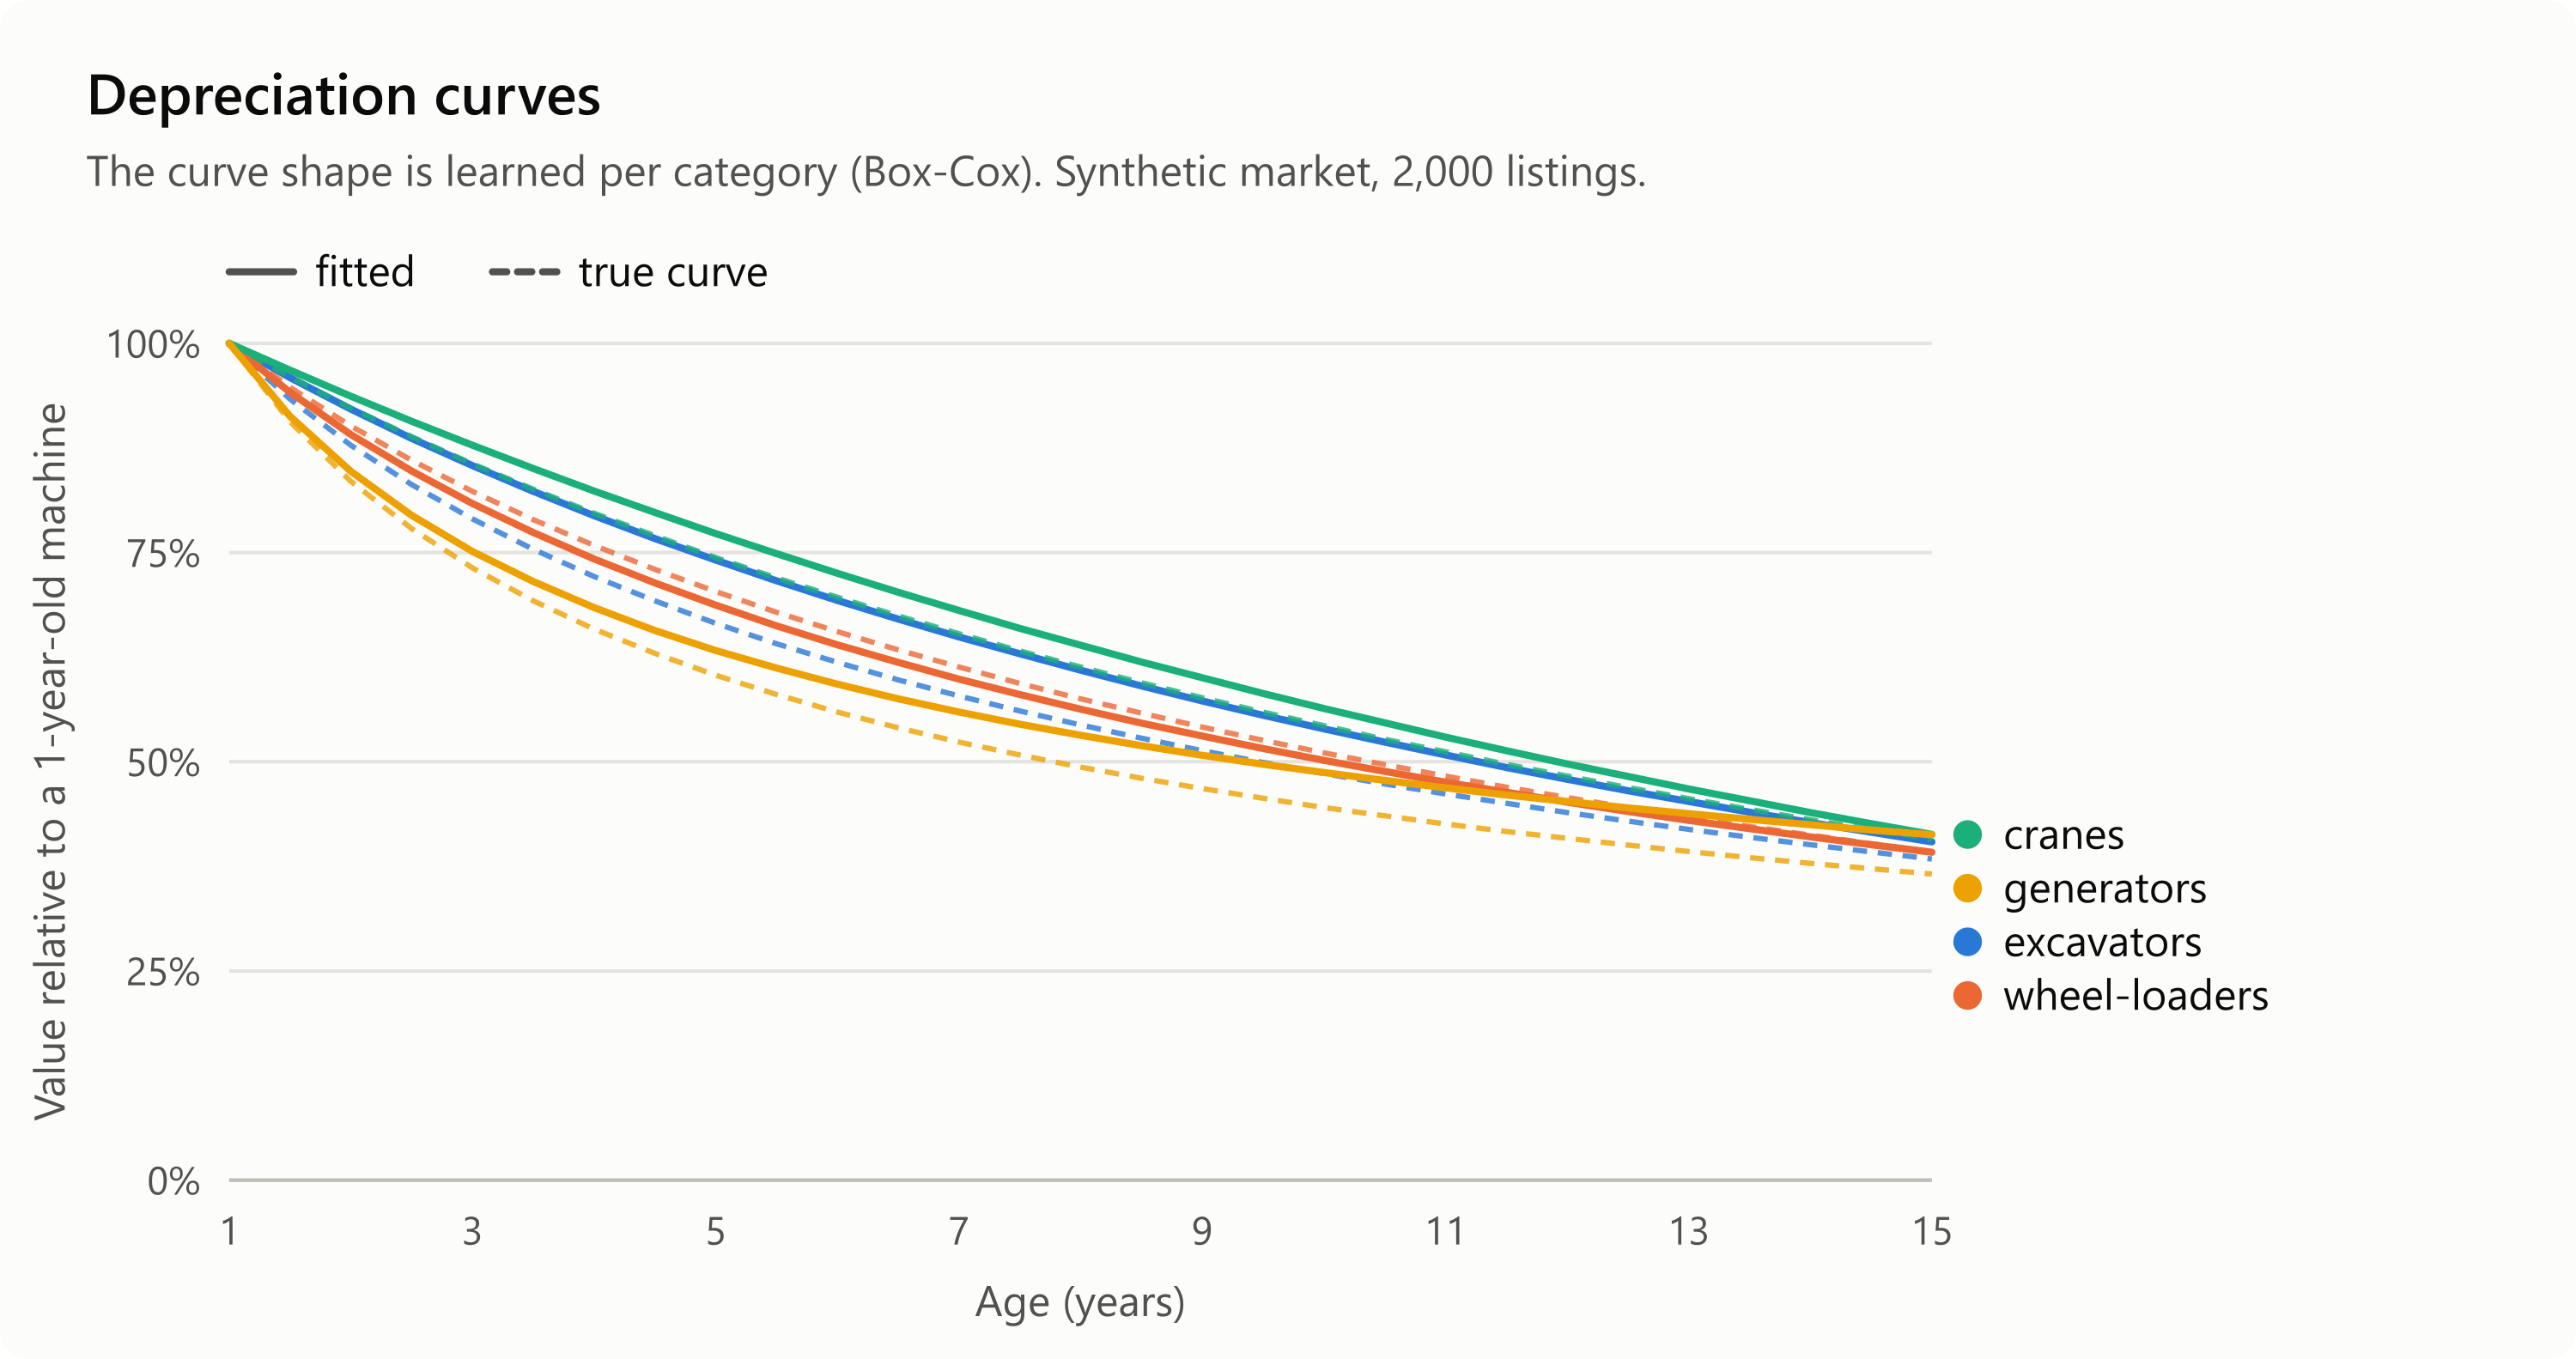
\includegraphics[width=0.49\linewidth]{figures/depreciation.png}\hfill
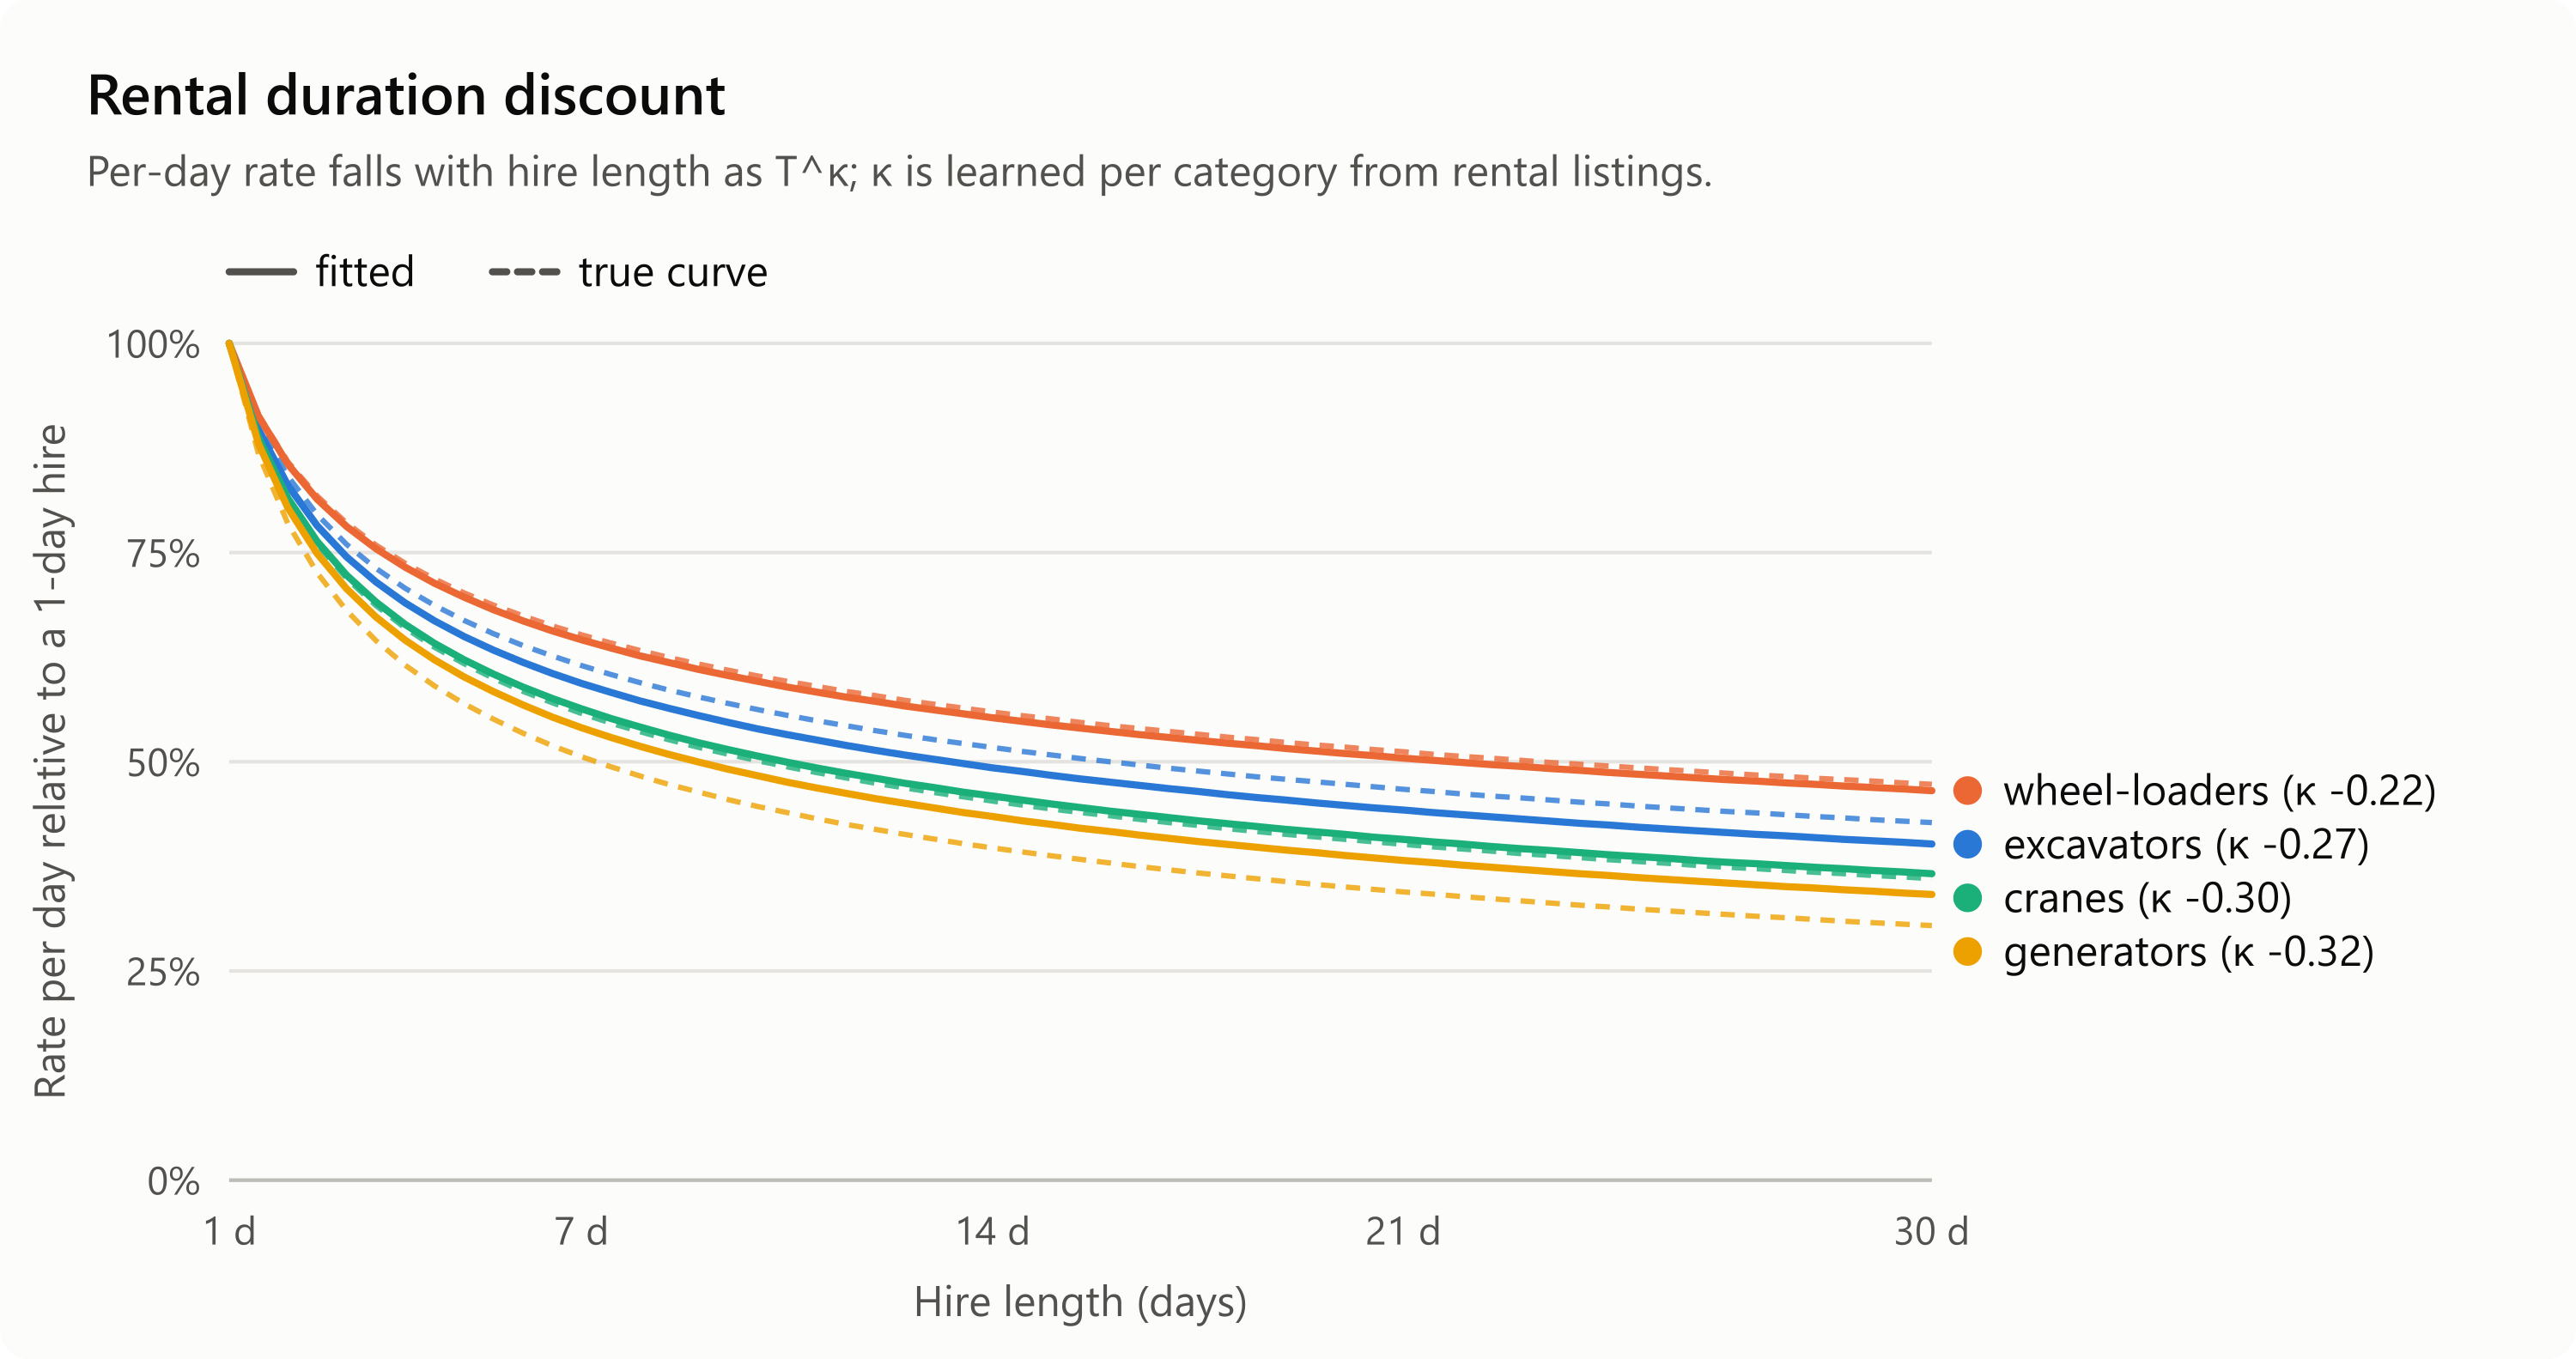
\includegraphics[width=0.49\linewidth]{figures/duration.png}
\caption{Fitted (solid) and true (dashed) depreciation curves (left) and rental duration discounts
(right) for four categories of one synthetic market of 2{,}000 listings.}
\label{fig:curves}
\end{figure}

Figure~\ref{fig:curves} shows the fitted curves of one market against the truth. The duration
discount is recovered almost exactly; the depreciation curves follow the true ones within the
spread of the data, with the noisier shape estimates visible in the first years.

\subsection{Accuracy and market size}
Table~\ref{tab:size} compares the models as the number of listings per category and side grows.

\begin{table}[t]
\centering\small
\caption{Median absolute percentage error (\%) by listings per category and side; four-fold cross-validation, mean over three markets. Best per side in bold.}
\label{tab:size}
\begin{tabular}{rccccccc}
\toprule
 & \multicolumn{4}{c}{Sale prices} & \multicolumn{3}{c}{Rental rates} \\
\cmidrule(lr){2-5}\cmidrule(lr){6-8}
$n$ & Median & \textsc{sherpa-0} & OLS & \textsc{sherpa-1} & Median & OLS & \textsc{sherpa-1} \\
\midrule
20 & 46.2 & 33.6 & 45.4 & \textbf{30.6} & 50.5 & 49.6 & \textbf{28.0} \\
40 & 53.1 & 35.9 & 38.1 & \textbf{31.4} & 50.8 & 44.3 & \textbf{28.4} \\
80 & 50.9 & 31.4 & 33.2 & \textbf{26.5} & 48.0 & 35.3 & \textbf{26.1} \\
160 & 50.2 & 30.0 & 29.4 & \textbf{24.2} & 45.5 & 30.0 & \textbf{23.9} \\
\bottomrule
\end{tabular}
\end{table}


\textsc{sherpa-1} has the lowest error at every market size, on both sides. The gap is largest in
small markets: with 20 listings per category and side, ordinary least squares is no better than the
category median (45.4\% against 46.2\% on sale prices), while \textsc{sherpa-1} reaches 30.6\%; on
rental rates the difference is 49.6\% against 28.0\%. With 160 listings the hedonic regression has
enough data for its many dummy variables and closes most of the gap (29.4\% against 24.2\% on sale
prices). \textsc{sherpa-0} is competitive with ordinary least squares on sale prices but cannot
price rentals.


\subsection{Robustness}
Table~\ref{tab:robust} varies the share of impossible prices and the share of empty fields.

\begin{table}[t]
\centering\small
\caption{Robustness: MdAPE (\%) with 80 listings per category and side, mean over three markets. Models are trained on the raw listings; scored on held-out listings with plausible prices.}
\label{tab:robust}
\begin{tabular}{lcccccc}
\toprule
 & \multicolumn{3}{c}{Sale prices} & \multicolumn{3}{c}{Rental rates} \\
\cmidrule(lr){2-4}\cmidrule(lr){5-7}
Condition & Median & OLS & \textsc{sherpa-1} & Median & OLS & \textsc{sherpa-1} \\
\midrule
0\% impossible prices & 50.8 & \textbf{26.3} & 27.2 & 46.6 & 28.8 & \textbf{27.4} \\
5\% impossible prices & 51.0 & 42.0 & \textbf{27.0} & 47.8 & 42.4 & \textbf{27.6} \\
10\% impossible prices & 50.8 & 51.0 & \textbf{26.2} & 48.9 & 51.8 & \textbf{27.6} \\
20\% impossible prices & 51.4 & 64.6 & \textbf{27.8} & 48.1 & 66.7 & \textbf{27.9} \\
\midrule
10\% empty fields & 48.8 & 31.9 & \textbf{24.3} & 48.4 & 32.4 & \textbf{24.5} \\
30\% empty fields & 48.8 & 35.9 & \textbf{31.3} & 48.4 & 36.3 & \textbf{29.5} \\
50\% empty fields & 48.8 & 41.6 & \textbf{36.9} & 48.4 & 38.3 & \textbf{33.2} \\
\bottomrule
\end{tabular}
\end{table}


On clean synthetic data the regression and \textsc{sherpa-1} are level (26.3\% and 27.2\%, within
one standard error). A share of impossible prices---placeholders, a missing or extra factor of
1{,}000---is where they part: 5\% of such prices raise the regression's error to 42\%, 20\% to
65\%, worse than the category median, while \textsc{sherpa-1} stays at 26--28\% because its cleaning
step and median-based estimates ignore them. As fields are left empty, every model degrades, but
\textsc{sherpa-1} keeps its lead (36.9\% against 41.6\% on sale prices with half of all fields
empty).


\subsection{Rental listings help sale estimates}
Table~\ref{tab:joint} holds 160 rental listings per category and varies the sale listings.

\begin{table}[t]
\centering\small
\caption{Sale-price MdAPE (\%) with 160 rental listings per category and few sale listings; mean over five markets. \textit{Sale only} fits \textsc{sherpa-1} without the rental listings.}
\label{tab:joint}
\begin{tabular}{rcccc}
\toprule
Sale listings per category & Median & \textsc{sherpa-1}, sale only & \textsc{sherpa-1}, joint & Gain (points) \\
\midrule
10 & 54.5 & 42.7 & \textbf{31.9} & 10.8 \\
20 & 54.8 & 37.3 & \textbf{31.5} & 5.8 \\
40 & 51.1 & 30.9 & \textbf{27.0} & 3.8 \\
\bottomrule
\end{tabular}
\end{table}


Rental listings improve sale estimates, and most where sales are scarce. With 10 sale listings per
category, fitting the 160 rental listings jointly lowers the sale-price error from 42.7\% to 31.9\%;
with 20 from 37.3\% to 31.5\%; with 40 from 30.9\% to 27.0\%. The rental listings carry information
about the depreciation curve, size, condition and brand effects that the shared value core passes
to the sale side.


\subsection{Interval calibration}

\begin{table}[t]
\centering\small
\caption{Share (\%) of held-out prices inside the 50\% and 80\% intervals; four-fold cross-validation, mean over three markets. Nominal levels: 50 and 80.}
\label{tab:coverage}
\begin{tabular}{rlcccc}
\toprule
 & & \multicolumn{2}{c}{Sale} & \multicolumn{2}{c}{Rent} \\
\cmidrule(lr){3-4}\cmidrule(lr){5-6}
$n$ & Intervals & 50\% & 80\% & 50\% & 80\% \\
\midrule
40 & conformal & 57.1 & 86.6 & 57.1 & 86.4 \\
40 & normal & 44.3 & 73.2 & 42.5 & 69.2 \\
160 & conformal & 52.1 & 82.9 & 52.6 & 83.0 \\
160 & normal & 54.3 & 83.5 & 53.7 & 81.7 \\
\bottomrule
\end{tabular}
\end{table}


Table~\ref{tab:coverage} compares cross-conformal intervals with normal intervals of the same
scale. In small markets (40 listings per category and side) normal intervals under-cover---44\% and
73\% of held-out sale prices fall inside the nominal 50\% and 80\% intervals---because the robust
scale is estimated from few residuals and missing inputs add error the scale does not see. The
conformal intervals are conservative instead (57\% and 87\%). With 160 listings both are close to
nominal (52--54\% and 82--84\%). Conformal calibration thus matters most where data are thin, which
is the setting \sherpa{} is designed for.


\subsection{Ablations}
Figure~\ref{fig:ablation} switches off one block at a time on a market of 1{,}200 listings.

\begin{figure}[t]
\centering
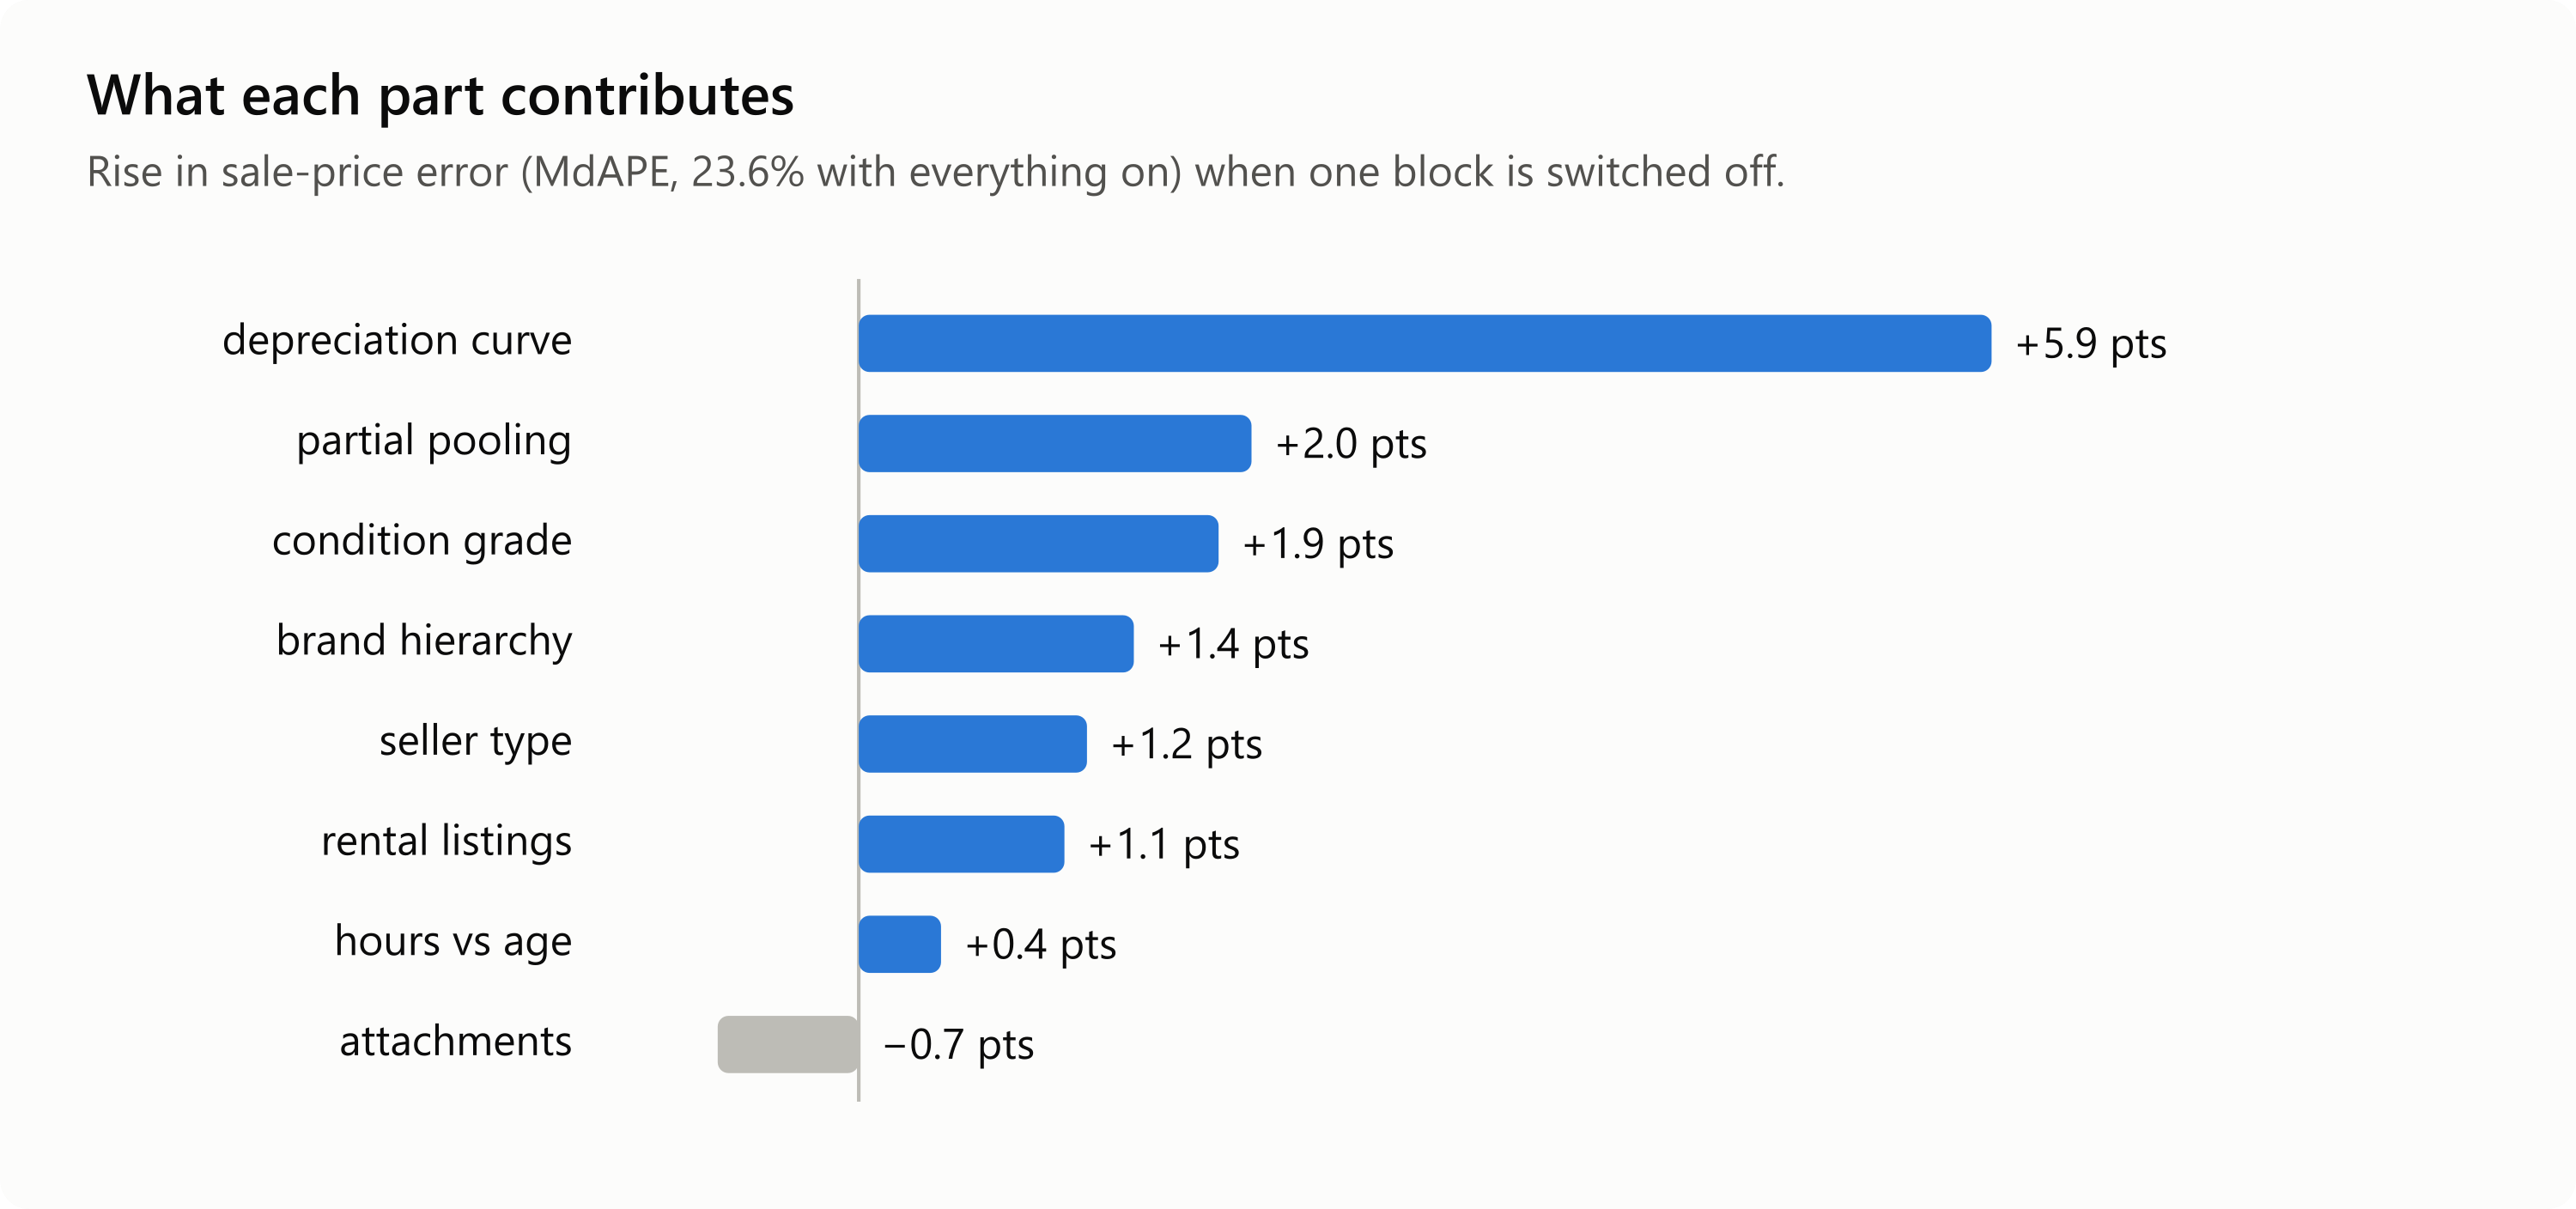
\includegraphics[width=0.85\linewidth]{figures/ablation.png}
\caption{Rise in sale-price MdAPE when one block of \sherpa{} is switched off (five-fold
cross-validation, 1{,}200 synthetic listings).}
\label{fig:ablation}
\end{figure}

The flexible depreciation curve contributes most (+5.9 points of MdAPE when replaced by a fixed
curve), followed by partial pooling (+2.0), condition grade (+1.9), the brand hierarchy (+1.4),
seller type (+1.2) and the joint fit of rental listings (+1.1). Attachment effects in this market are
small (3--10\% of value on a quarter of listings) and estimating them costs slightly more than it
gains ($-0.7$).

\section{Discussion}
\label{sec:discussion}

\paragraph{What the joint model buys.}
Sharing the value core lets each side of the market inform the other. The gain is largest where
it matters most in practice: categories that are often hired and rarely sold.

\paragraph{Weakly identified parameters.}
New machines are listed at age~0 and used machines from about one year, so listings cannot separate
the premium of a new machine from the curvature of the depreciation curve in its first year. In the
simulations $\lambda$ is unbiased on average but noisy (RMSE 0.32) and $\theta$ is biased upward
(+0.14), while the ten-year depreciation $D$ is recovered without bias. The two parameters should be
interpreted together; the estimated value of a new machine is a safer summary than $\theta$ alone.

\paragraph{Numerical stability.}
Medians are step functions, so the fit responds to tiny perturbations by small jumps. With averaged
iterates, a relative change of $10^{-9}$ to every price moves predictions by a median of 0.3\%; the
TypeScript and Python implementations agree to the last digit for three rounds and within the same
margin thereafter.

\paragraph{Limitations.}
\sherpa{} models asking prices and rates, not transaction prices; the gap requires transaction data
\citep[cf.][]{han2016}. Listings without a price are not missing at random. The conformal guarantee
assumes exchangeability, which strong market trends weaken. All results here are on synthetic data
drawn from the model's own form, which favours the model; the comparison with ordinary least squares
measures the value of robustness, pooling and joint fitting, not of the functional form. A case
study on real listings, and comparisons with gradient-boosted trees, are planned for the next
version.

\section{Software and reproducibility}
\label{sec:software}

\sherpa{} is available under the Apache License~2.0 at
\url{https://github.com/dev-kakosoai/sherpa-valuation}. Release v0.1.0 contains a TypeScript
package (\texttt{@equipmentsfinder/sherpa}) and a Python package (\texttt{sherpa-valuation}).
Neither has runtime dependencies; listings and fitted models are plain JSON in both, and a
cross-language test keeps the implementations equal. Every number in this paper is produced by
the scripts \texttt{bench/paper.ts} and \texttt{bench/benchmark.ts} in that repository.

\section*{Acknowledgements}
\sherpa{} was developed at EquipmentsFinder (\url{https://www.equipmentsfinder.com}), a marketplace
for heavy equipment in the United Arab Emirates and Saudi Arabia, whose listings motivated its
design.

\bibliographystyle{plainnat}
\bibliography{references}

\appendix
\section{Parameters of the synthetic markets}
\label{app:truth}
\begin{table}[h]
\centering\small
\caption{Category parameters of the synthetic markets. $D$ is the log-value change from new to age 10; $\pi$ is given as the daily rate per unit of value, $e^{\pi}$.}
\begin{tabular}{lrrrrrrrrrr}
\toprule
Category & Base price & $D$ & $\lambda$ & $\gamma$ & $\delta$ & $\theta$ & $\zeta$ & $e^{\pi}$ & $\kappa$ & $\omega$ \\
\midrule
excavators & 300,000 & $-$0.90 & 0.40 & 0.70 & $-$0.15 & 0.20 & 0.30 & 0.0013 & $-$0.25 & 0.35 \\
wheel-loaders & 260,000 & $-$0.80 & 0.60 & 0.60 & $-$0.12 & 0.18 & 0.25 & 0.0012 & $-$0.22 & 0.30 \\
cranes & 900,000 & $-$0.70 & 0.80 & 0.80 & $-$0.10 & 0.15 & 0.15 & 0.0011 & $-$0.30 & 0.25 \\
generators & 60,000 & $-$1.10 & 0.10 & 0.55 & $-$0.20 & 0.22 & 0.00 & 0.0025 & $-$0.35 & 0.00 \\
compactors & 45,000 & $-$0.85 & 0.50 & 0.00 & $-$0.10 & 0.15 & 0.20 & 0.0018 & $-$0.28 & 0.20 \\
\bottomrule
\end{tabular}

\vspace{0.6em}
Grade: 1: $-$0.45, 2: $-$0.18, 3: 0.00, 4: 0.12.
Attachments: bucket 0.03, breaker 0.10, coupler 0.04, forks 0.05.
Seller: dealer 0.10, rental $-$0.04, private $-$0.06.
Origin: japan 0.08, europe 0.06, usa 0.05, korea $-$0.03, china $-$0.20.
Emissions: tier2 $-$0.10, tier3 0.00, tier4i 0.05, tier4f 0.10.
Inspection 0.06; market trend 0.004 per month; time on market 0.04; completeness 0.08.
Noise standard deviation 0.22--0.30 on log price, by category.
\end{table}


\end{document}
